\subsubsection{SNL ATDM Programming Models: Kokkos} 

\paragraph{Overview} 
Kokkos provides a C++ Parallel Programming Model for Performance Portability. 
It is implemented as a C++ abstraction layer over existing parallel programming models such as OpenMP, CUDA and C++ std::threads. 
Application and library developers can implement their code using Kokkos, 
which will map their parallel algorithms onto the underlying execution mechanism. 
Codes written in that manner can then be compiled to run on each current HPC platform, including CPU and GPU based systems.
Furthermore, new types of architectures generally need only be added to Kokkos, while no changes are necessary to end applications - even if the new architecture requires its own custom programming mechanism. 

\paragraph{Key  Challenges}
Teams of scientists, engineers, and mathematicians apply their specific expertise to develop application software 
to solve problems from their specialized domains. 
The largest and most complex of these require the use of High Performance Computing (HPC). 
For more than two decades, HPC applications used parallel computing on a network of compute-nodes 
consisting of a computer chip with either a single core or very few processing cores 
and memory dedicated to each core. 
However, the “many-core revolution,” which has slowly arisen in the last five years, 
has dramatically changed the nature of HPC because processors in modern compute-nodes 
have many cores that must share the compute-node’s memory.

The many-core revolution in computing is characterized by: 
(1) a steady increase in the number of cores within individual computer chips; 
(2) a corresponding decrease in the amount of memory per core that must be shared by the cores of a chip, and, 
(3), the diversity of computer chip architectures. 
This diversity is highly disruptive because each architecture imposes different complex 
and sometimes conflicting requirements on software to perform well on an architecture. 
Application software development teams are confronted with the dual challenges of: 
(1) inventing new parallel algorithms for many-core chips, 
(2) learning the different programming mechanisms of each architecture, and
(2), creating and maintaining separate versions of their software specialized for each architecture. 
These tasks may involve considerable overhead for organizations in terms of time and cost. 
Adapting application software to changing HPC requirements is already becoming a large expense for 
HPC users and can be expected to grow as the diversity of HPC architectures continues to rise.
An alternative, however, is creating software that is performance portable across current and future architectures. 

A key issue for achieving performance portability is, that one does not only need to address parallel execution but also data management. 
This includes the handling of memory hierarchies consisting of resources such as HBM, DDR and NVM memory as well as the question of memory layouts, which might need to be different for various architectures. 

\paragraph{Solution Strategy}

The Kokkos project developed a parallel programming model with flexible enough semantics that it can be mapped on a diverse set of HPC architectures including current multi-core CPUs and massively parallel GPUs. 
The programming model is implemented using C++ template abstractions, which allow a compile time translation to the underlying programming mechanism on each platform, using their respective primary tool chains. 
Compared to approaches which rely on source-to-source translators or special compilers, this way leverages the investment of vendors in their preferred programming mechanism without introducing additional, hard to maintain, tools in the compilation chain. 

\begin{figure}[ht!]
\centering
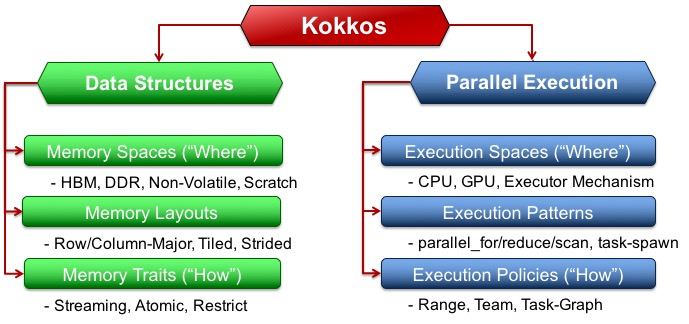
\includegraphics[width=90mm]{projects/2.3.1-PMR/2.3.1.04-SNL-ATDM-PMR/kokkos-abstractions.jpg}
\caption{Kokkos Execution and Memory Abstractions}
\end{figure}

Applications written in Kokkos are leveraging its six core abstractions for parallel execution and data management. 
These abstractions provide the flexibility to allow the mapping of execution and data to the diverse set of architectures. 
As an example the "parallel\_for" Execution Pattern does neither guarantee order of execution nor concurrency of execution. 
That allows Kokkos to use threading, vectorization or even pipelining of operations to parallelize the algorithm. 

The Parallel Execution abstractions are (1) Execution Patterns, (2) Execution Policies, and (3) Execution Spaces. 
{\it Execution Patterns} describe what fundamental parallel algorithm is performed. This includes parallel loops, parallel reductions, and parallel scans as well as task spawn operations. 
{\it Execution Policies} control how the patterns are executed. They for example control the iteration space and whether scheduling is done dynamically or statically.
{\it Execution Spaces} denote different resources to execute on such as GPU or CPU. 

The Memory abstractions are (1) Memory Layout, (2) Memory Traits, and (3) Memory Space). 
{\it Memory Layout} describes the mapping of logical indices to the actual memory address. 
This allows to change the data access pattern in an algorithm without changing the implementation of the algorithm.
{\it Memory Traits} describe access properties, such as whether the user wants to perform atomic accesses, or whether accesses are guaranteed non-aliased. 
{\it Memory Spaces} control where data is allocated. This allows users to access HBM and DDR memory as well as special Scratch Memory. 


As a programming model, Kokkos is highly invasive in any code it is used by. 
Consequently, software quality is a critical concern.
Kokkos addresses this through a comprehensive testing regime, which includes over 250 combinations of compilers, hardware platforms and backends which are run every night. 
These tests cover current production HPC environments as well as prototype environments for future systems. 

Kokkos is available to users under the BSD license, permitting use of Kokkos in other open source codes as well as closed source code. 
It is maintained and developed at {\it https://github.com/kokkos/kokkos}. 

\paragraph{Recent Progress}

Kokkos is now used by a wide number of applications at various institutions. 
This includes multiple DOE laboratories as well as universities and other HPC centers.
At Sandia National Laboratories Kokkos is the primary programming model to address support for GPU based platforms in a performance portable manner, and numerous production level applications are actively porting to using Kokkos. 
The SNL ATDM applications are largely demonstrating performance portability today for a subset of their capabilities and are working towards full fletched support of all HPC platforms. 

Recent advances in Kokkos include support for more portable and performant scatter-add type algorithms, dynamic and static task graph support as well as support for NIVDIA Volta and ARM CPU architectures. 
This enables Kokkos applications to run on the DOE Summit and Sierra machines, which are getting installed now as well as at the upcoming Vanguard ARM based machine to be installed at Sandia in Summer 2018. 
  
\paragraph{Next Steps}

The Kokkos team is working with the Path Forward vendors to enable support for their architectures. 
This notably includes a new backend, called ROCm, for AMD GPUs, which is primarily developed by AMD itself. 
Furthermore, improvements on the dynamic task graph execution on GPUs are planned, in order to reduce the task granularity necessary to make effective use for GPUs. 
